\documentclass[12pt]{article}
\usepackage{graphicx}
\usepackage{hyperref}
\usepackage{cite}
\usepackage{mdframed}
\usepackage{float} % for [H] anchoring method

\graphicspath{ {pngs/} }
\mdfsetup{nobreak=true}

\begin{document}
\title{CSE326 Semester Project Requirement Spec: Anttris}
\author{Chris Aikman\\Benji Cope\\Skyler Manzanares\\Hugo Rivera\\Sean Turner}
\maketitle
% abstract
\begin{abstract}
Lorem Ipsum
\end{abstract}
% overview
\section{Project Overview}\label{overview-SM}
Anttris is designed to be a game that offers both creative freedom and a competitive edge. The game revolves around solving puzzle cubes which are composed of different types of blocks. Each block has a special property allowing for sophisticated puzzles to be created. Players can solve the puzzle cubes by interacting with these blocks, doing things from removing blocks from the cube to setting off massive chains!

Anttris will include two different game-mode categories: competitive game modes, and single-player game modes. Single-player game modes will focus on clearing puzzle cubes with emphasis placed on efficiency of the solution or solution time. Competitive game modes shift the focus to solving cubes faster than an opponent.

One central game concept to Anttris is the ability to creat your own puzzle cubes. Players will be able to create puzzle cubes that they can use when playing competitively. The goal of the game here is no longer to simply solve a cube faster than your opponent; you now also want to \textsl{create} a puzzle that will confuse your opponent long enough to solve theirs first.
\subsection{Scope and Objectives}\label{scope-obj-CA}
Anttris is a simple puzzle game idea that has many elements that can be extended after completion of the core gameplay. The project’s scope involves creating self-contained executables that work on many different platforms (including, but not limited to, PC, Mac, Linux) and can connect to other players through direct connection and, with enough time, through a random connection process involving a host server. In order to complete the project, we must utilize a game development framework that will provide the basic functionality of a 3-dimensional game. To further extend the scope, the game will need to use networking methods to connect two players together for competitive games. The objectives for the project have been planned in a way that the core gameplay mechanics can be completed on their own and will give a functional and complete game in itself. If the core of the project is completed ahead of schedule, then further objectives have been set in place that will allow for the additional of many neat and unique features that will add to the game’s fun and replayability factors. The main objectives of the project involve:
\begin{itemize}
 \item Completing core gameplay mechanics. This involves completing a single-player game that uses user input to manipulate the game’s state into winning the game.
 \item Completing graphical elements. This involves creating and modifying the visual elements of the game from the textures of the 3d objects to the graphical user interface.
 \item Completing multiplayer gameplay mechanics. This involves connecting to and communicating two individual players together on separate machines in order for the players to compete with each other on preset puzzle or puzzle they have made themselves.
 \item Adding additional gameplay mechanics. This involves adding on additional features that we may not have enough time to complete within the project’s timeline, but would like to if the base project is completed before scheduled. These ideas involve:
  \begin{itemize}
  \item Adding new block types.
  \item Adding online connections through a server setup instead of direct connection.
  \item Adding new competitive and single player game modes based on the same puzzle mechanics, such as ‘race the clock’ or ‘remove all blocks’.
  \end{itemize}
\end{itemize}
\subsection{Supplementary Requirements}\label{supplementary-reqs-SM}
% customer reqs
\subsubsection{Interface Requirements}
To make our video game easy to use, it is required that the user interface
provide intuitive interaction. To be able to make our game accessible to
the standard user, we have adopted as a requirement that standard
input devices -- namely a mouse -- be supported.

Graphical User Interfaces are to be simplistic, and not provide an overwhelming
volume of functionallity. Menu systems should contain no more than five (5)
functional options. Menus should follow a logical tree and \textsl{aid} in
game navigation.
\subsubsection{Performance Requirements}
As Anttris is to be professional-grade software, it is both necessary and
sufficient that it run quickly. As is the standard for video-games, Anttris
will deliver a minimum of 30 frames per second, and a max of 60 frames per
second. Any speed outside of this range on a modern-day computer is hereby
defined unacceptable.

%How do we define a modern day computer? regular old office computer?
As previously mentioned, Anttris is designed to be a game available to a common
computer user. To this end, the game is required to meet the above-defined
speed standard when tested on computers commonly used in a traditional office
workspace whose primary purpose is word-processing and web browsing.

\section{Customer Requirements}\label{cust-reqs-HR}
\subsection{User-Case Diagrams}
    \begin{figure}[H]
        \centering
        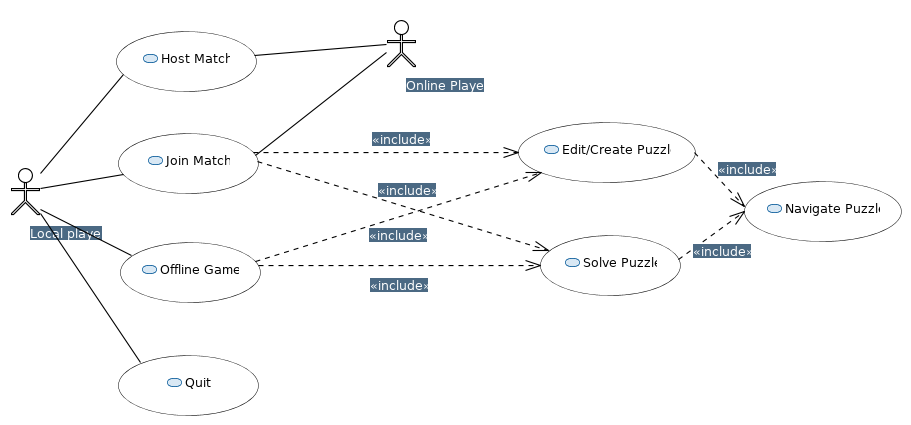
\includegraphics[width=6in]{use_cases.png}
        \caption{Use Case Diagram}
    \end{figure}

\subsection{Actor Descriptions}

\subsection{Use-case Descriptions}
\begin{mdframed}
    \subsubsection{Host match}
    \begin{description}
        \item[Entry conditions] Internet connection
        \item[Exit conditions] None. Will go back to game menu.
        \item[Participating Actors] Online player and local player
        \item[Flow of events]:
            \begin{enumerate}
                \item User creates a game, selects number of players and game
                    type
                \item User shares (friendly looking) match ID with other
                    players (I’m not sure about this…)
                \item These players may connect to the match
                \item The game ends when all players disconnect.
            \end{enumerate}
    \end{description}
\end{mdframed}

% reqs analysis
%\section{Requirements Analysis}\label{reqs-analysis-BC}

%\subsection{Scope and Objectives}

%\subsection{Supplementary Requirements}

% reqs analysis
\section{Requirements Analysis}

\subsection{Structural Analysis}\label{struct-analysis-BC}

\subsection{Behavioral Analysis}\label{behavioral-analysis-HR}

    \begin{figure}[H]
        \centering
        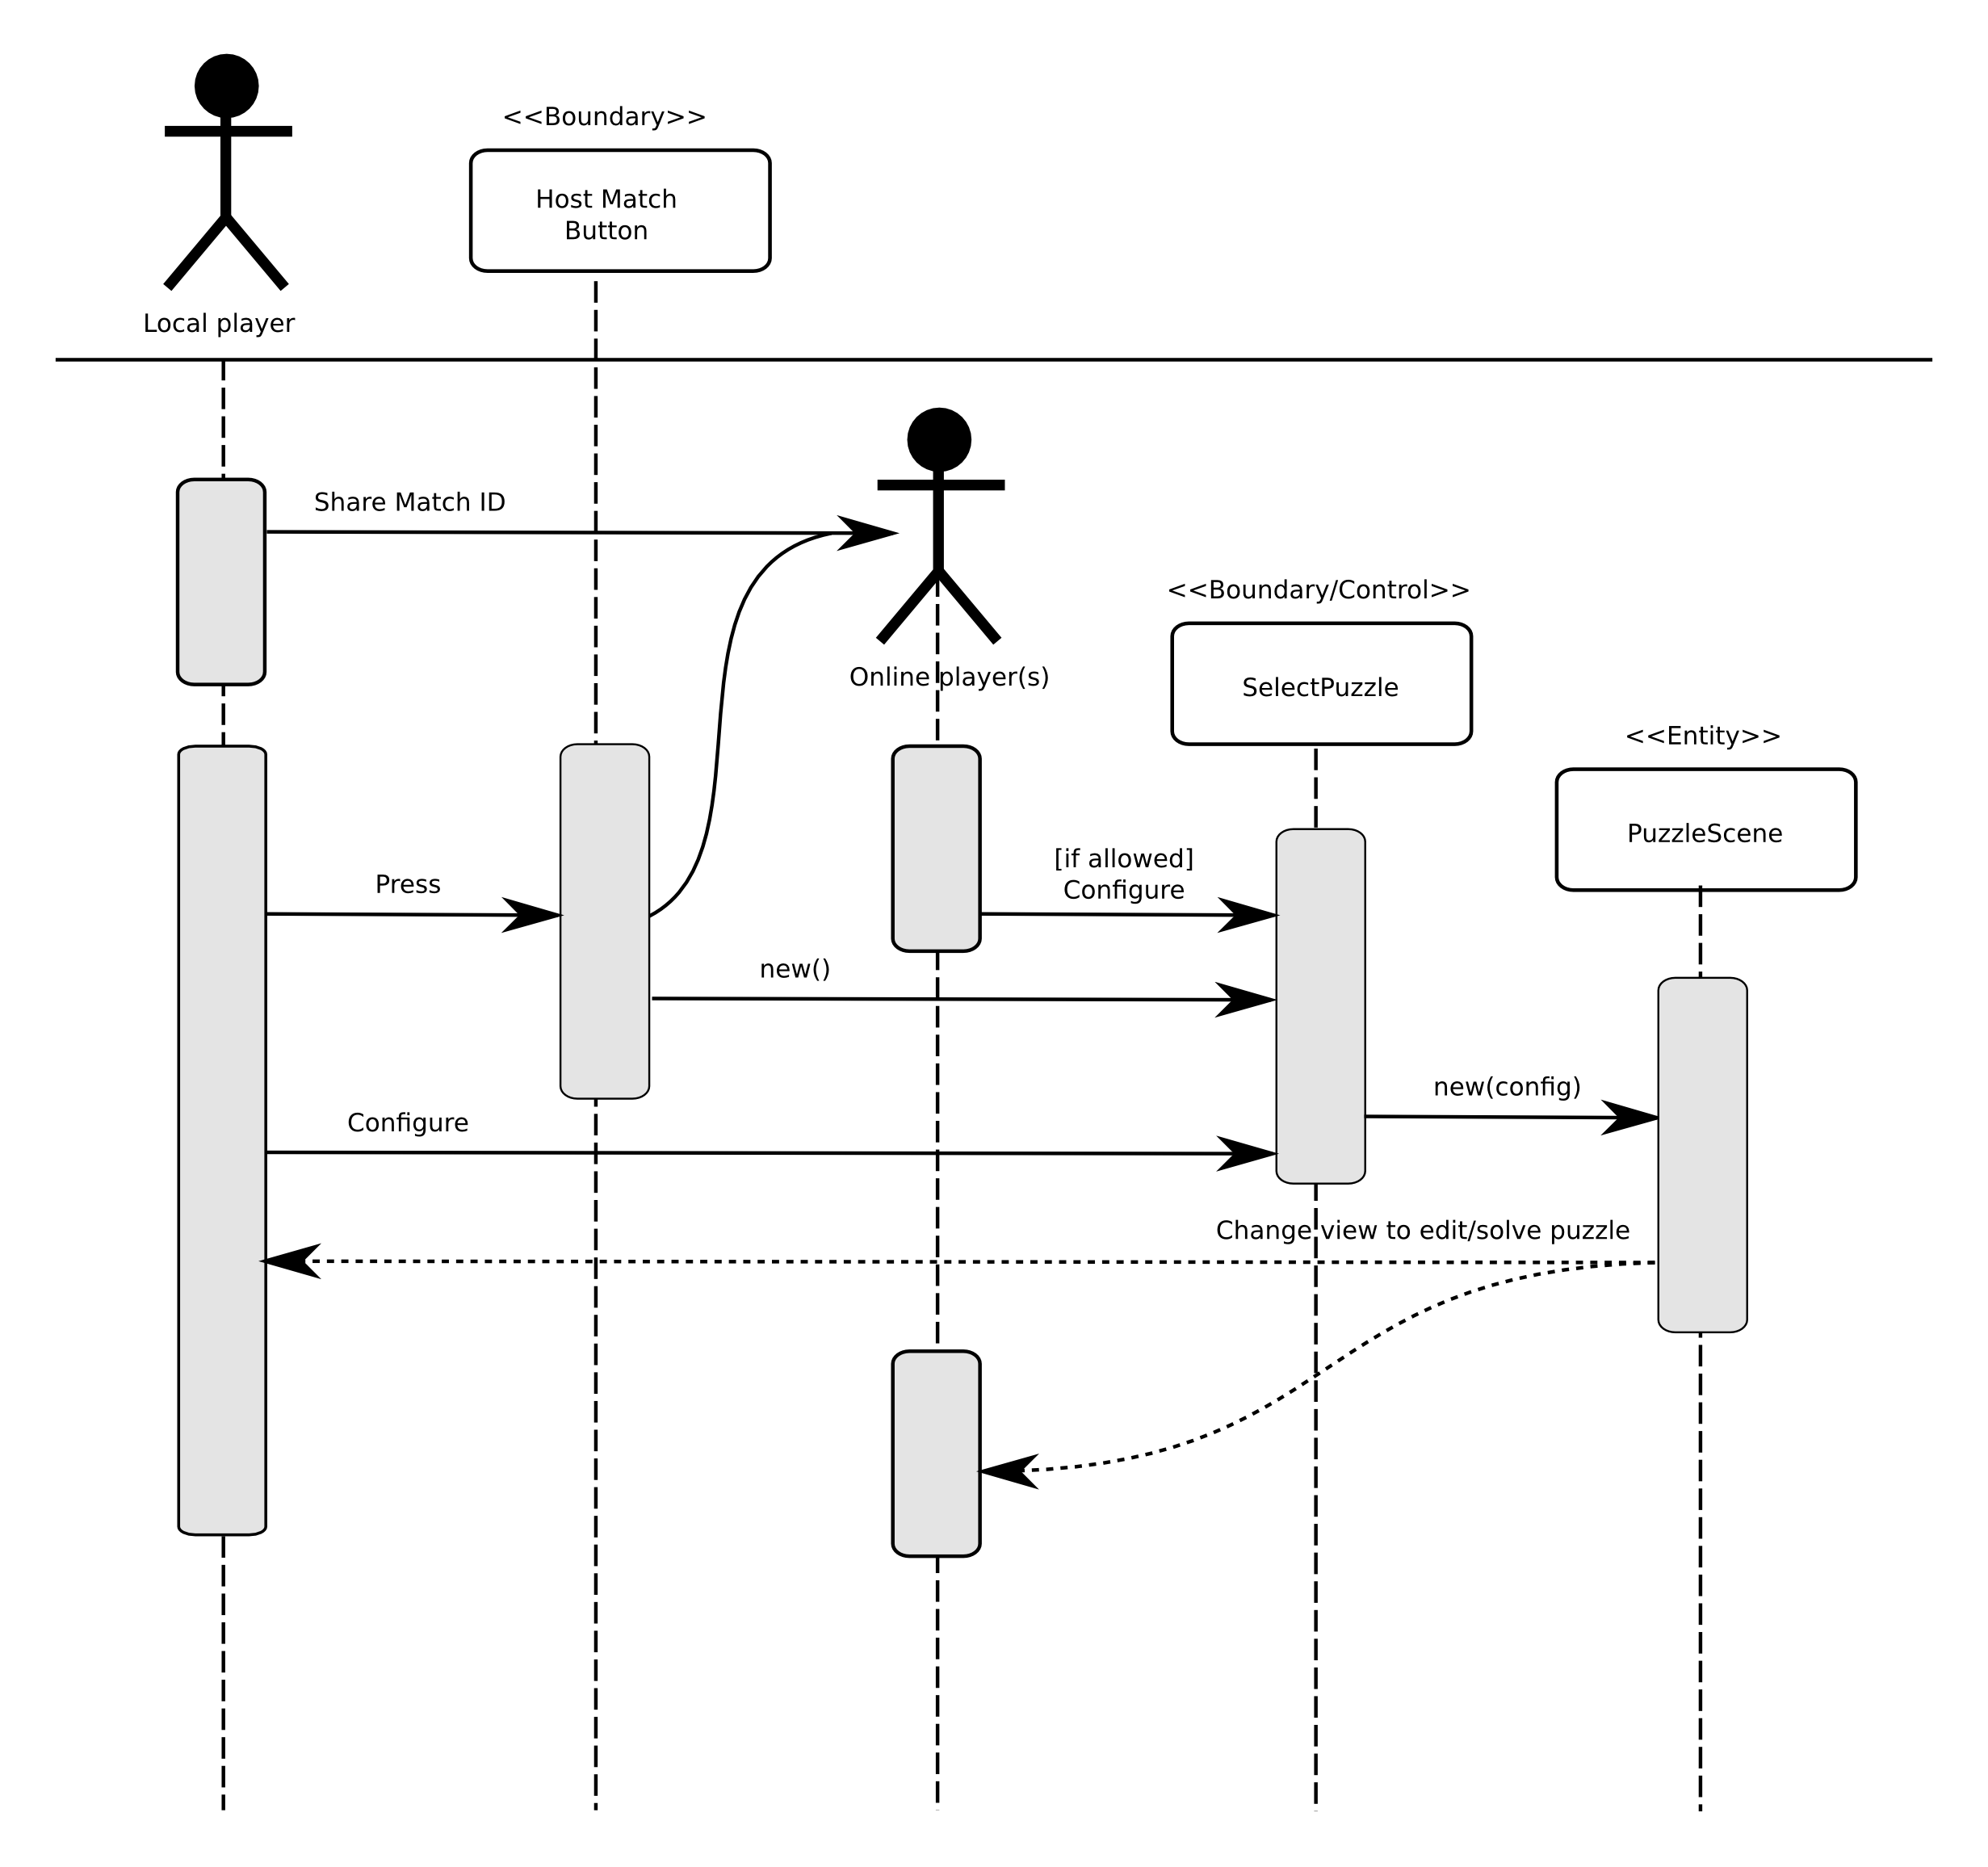
\includegraphics[width=6in]{sequence_host_match.png}
        \caption{UML Sequence Diagram for hosting a multiplayer game}
    \end{figure}


    \begin{figure}[H]
        \centering
        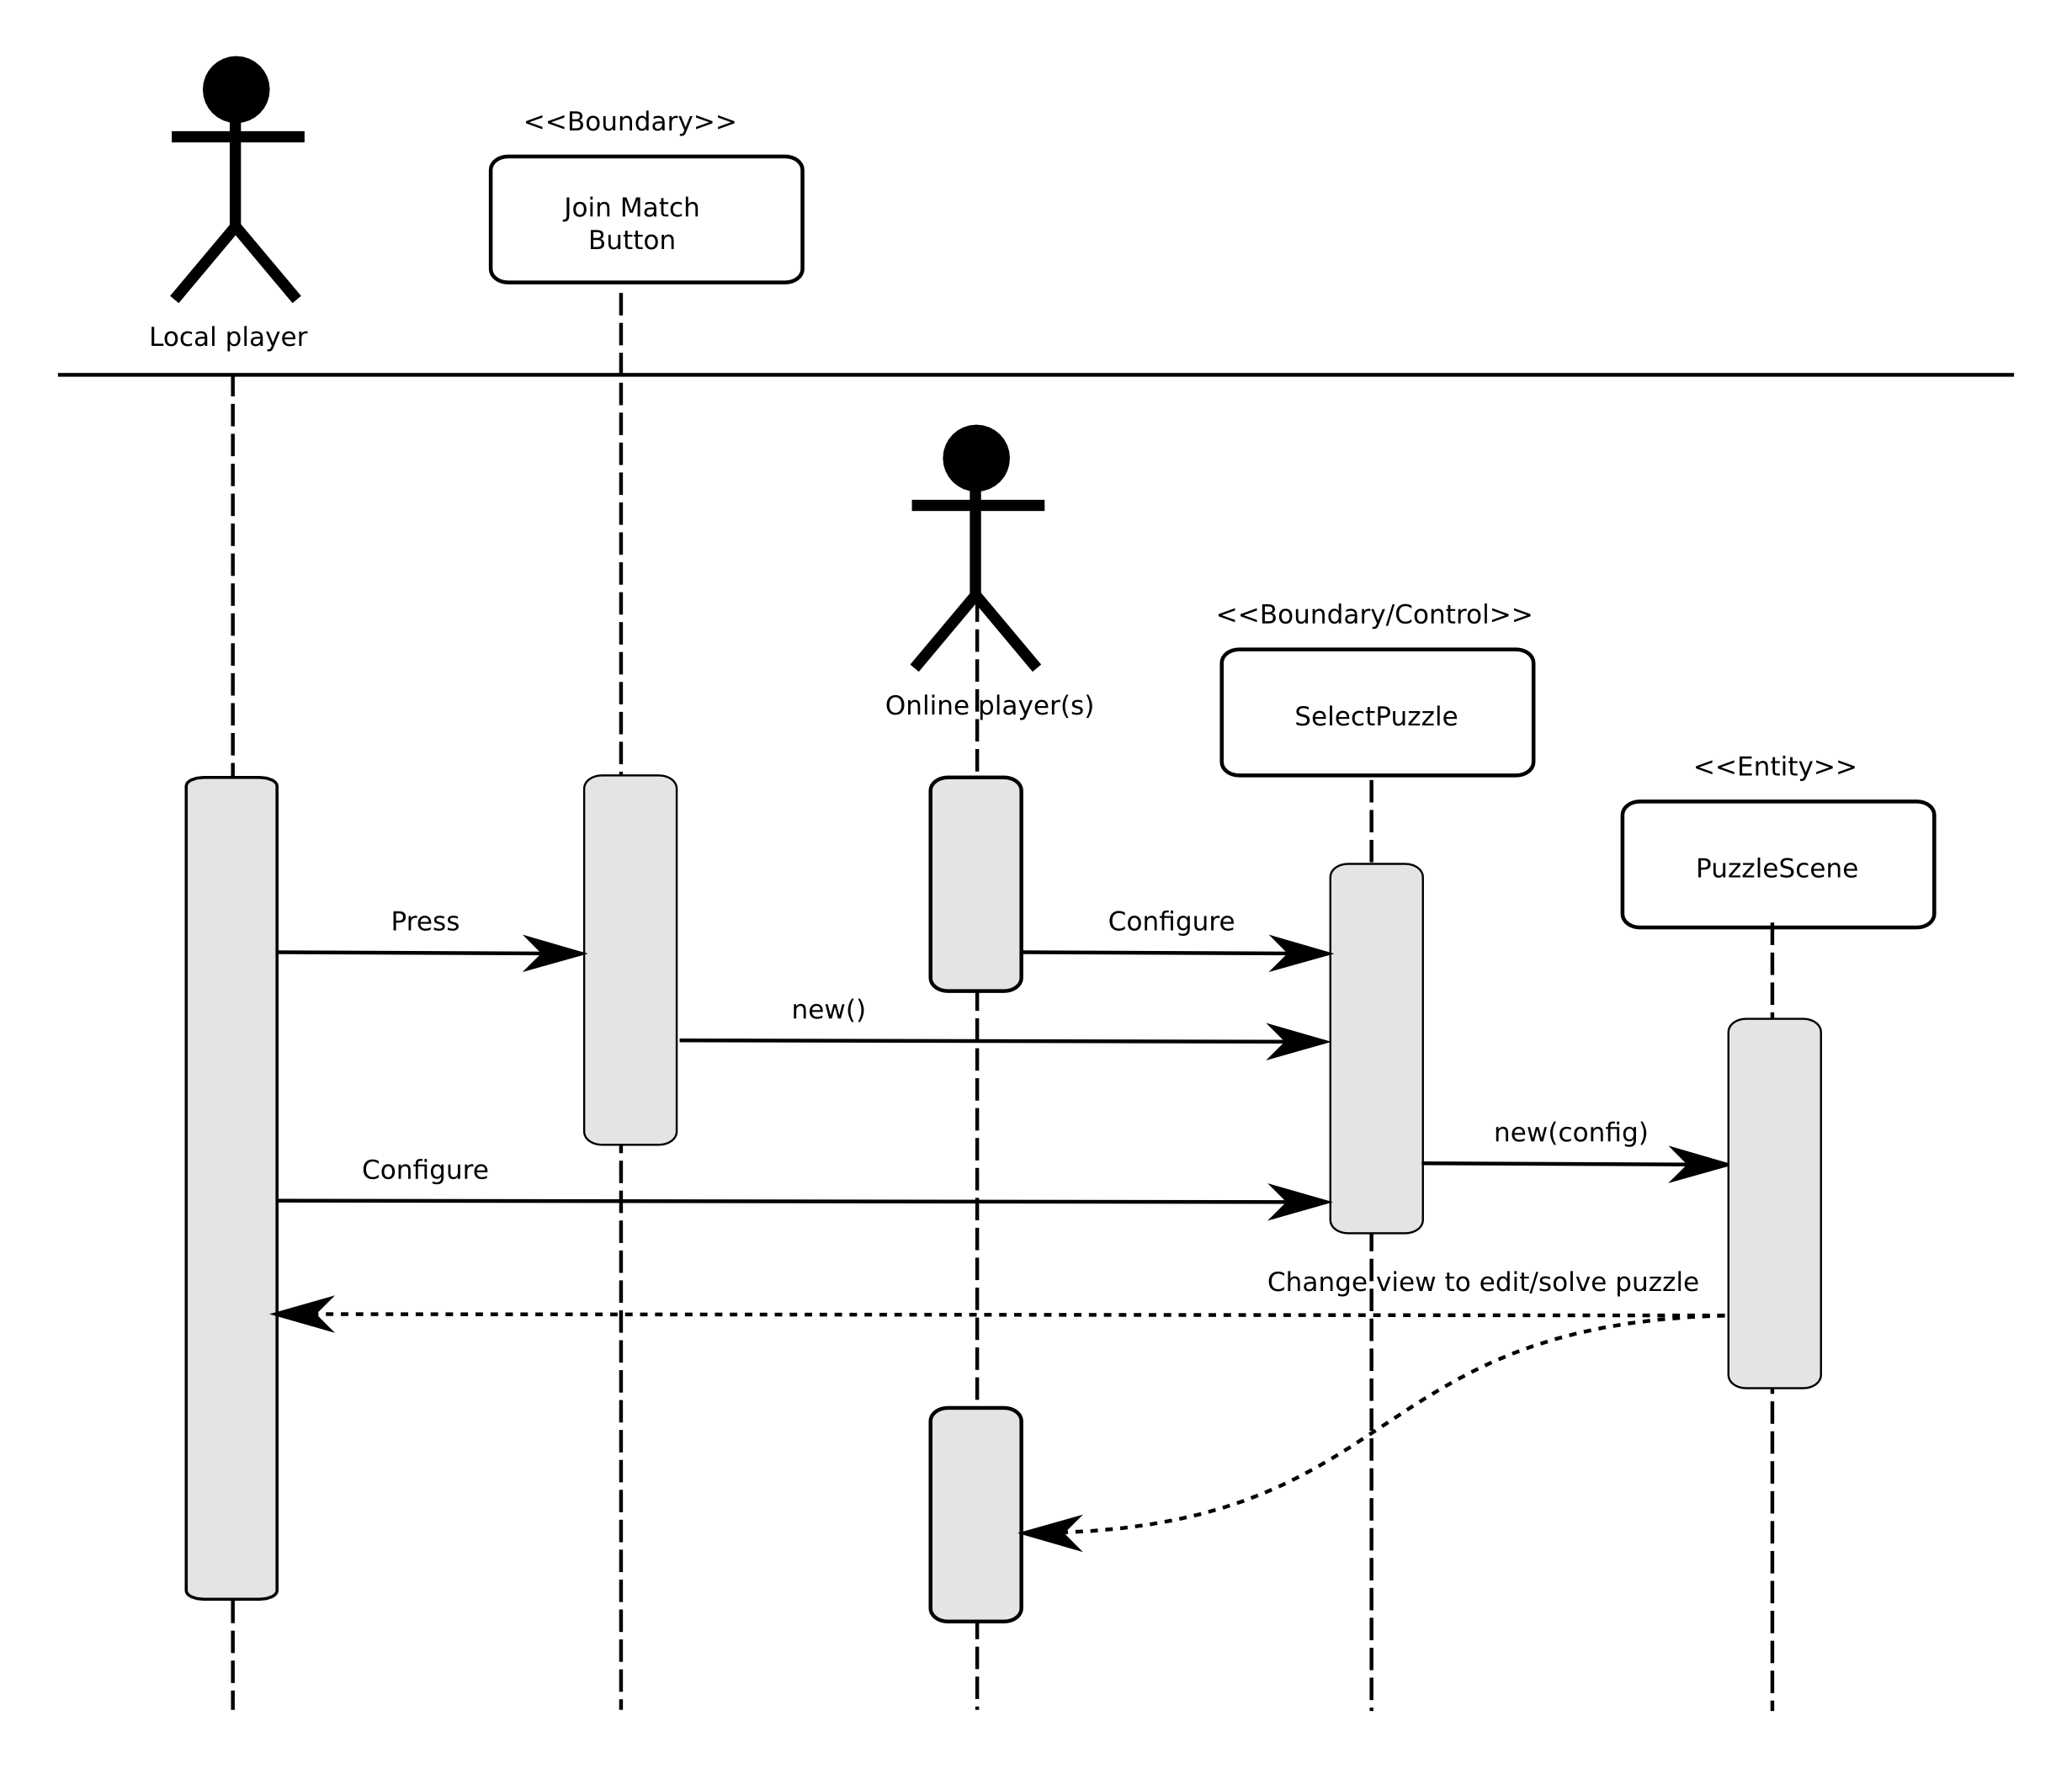
\includegraphics[width=6in]{sequence_join_match.png}
        \caption{UML Sequence Diagram for joining a multiplayer game}
    \end{figure}


    \begin{figure}[H]
        \centering
        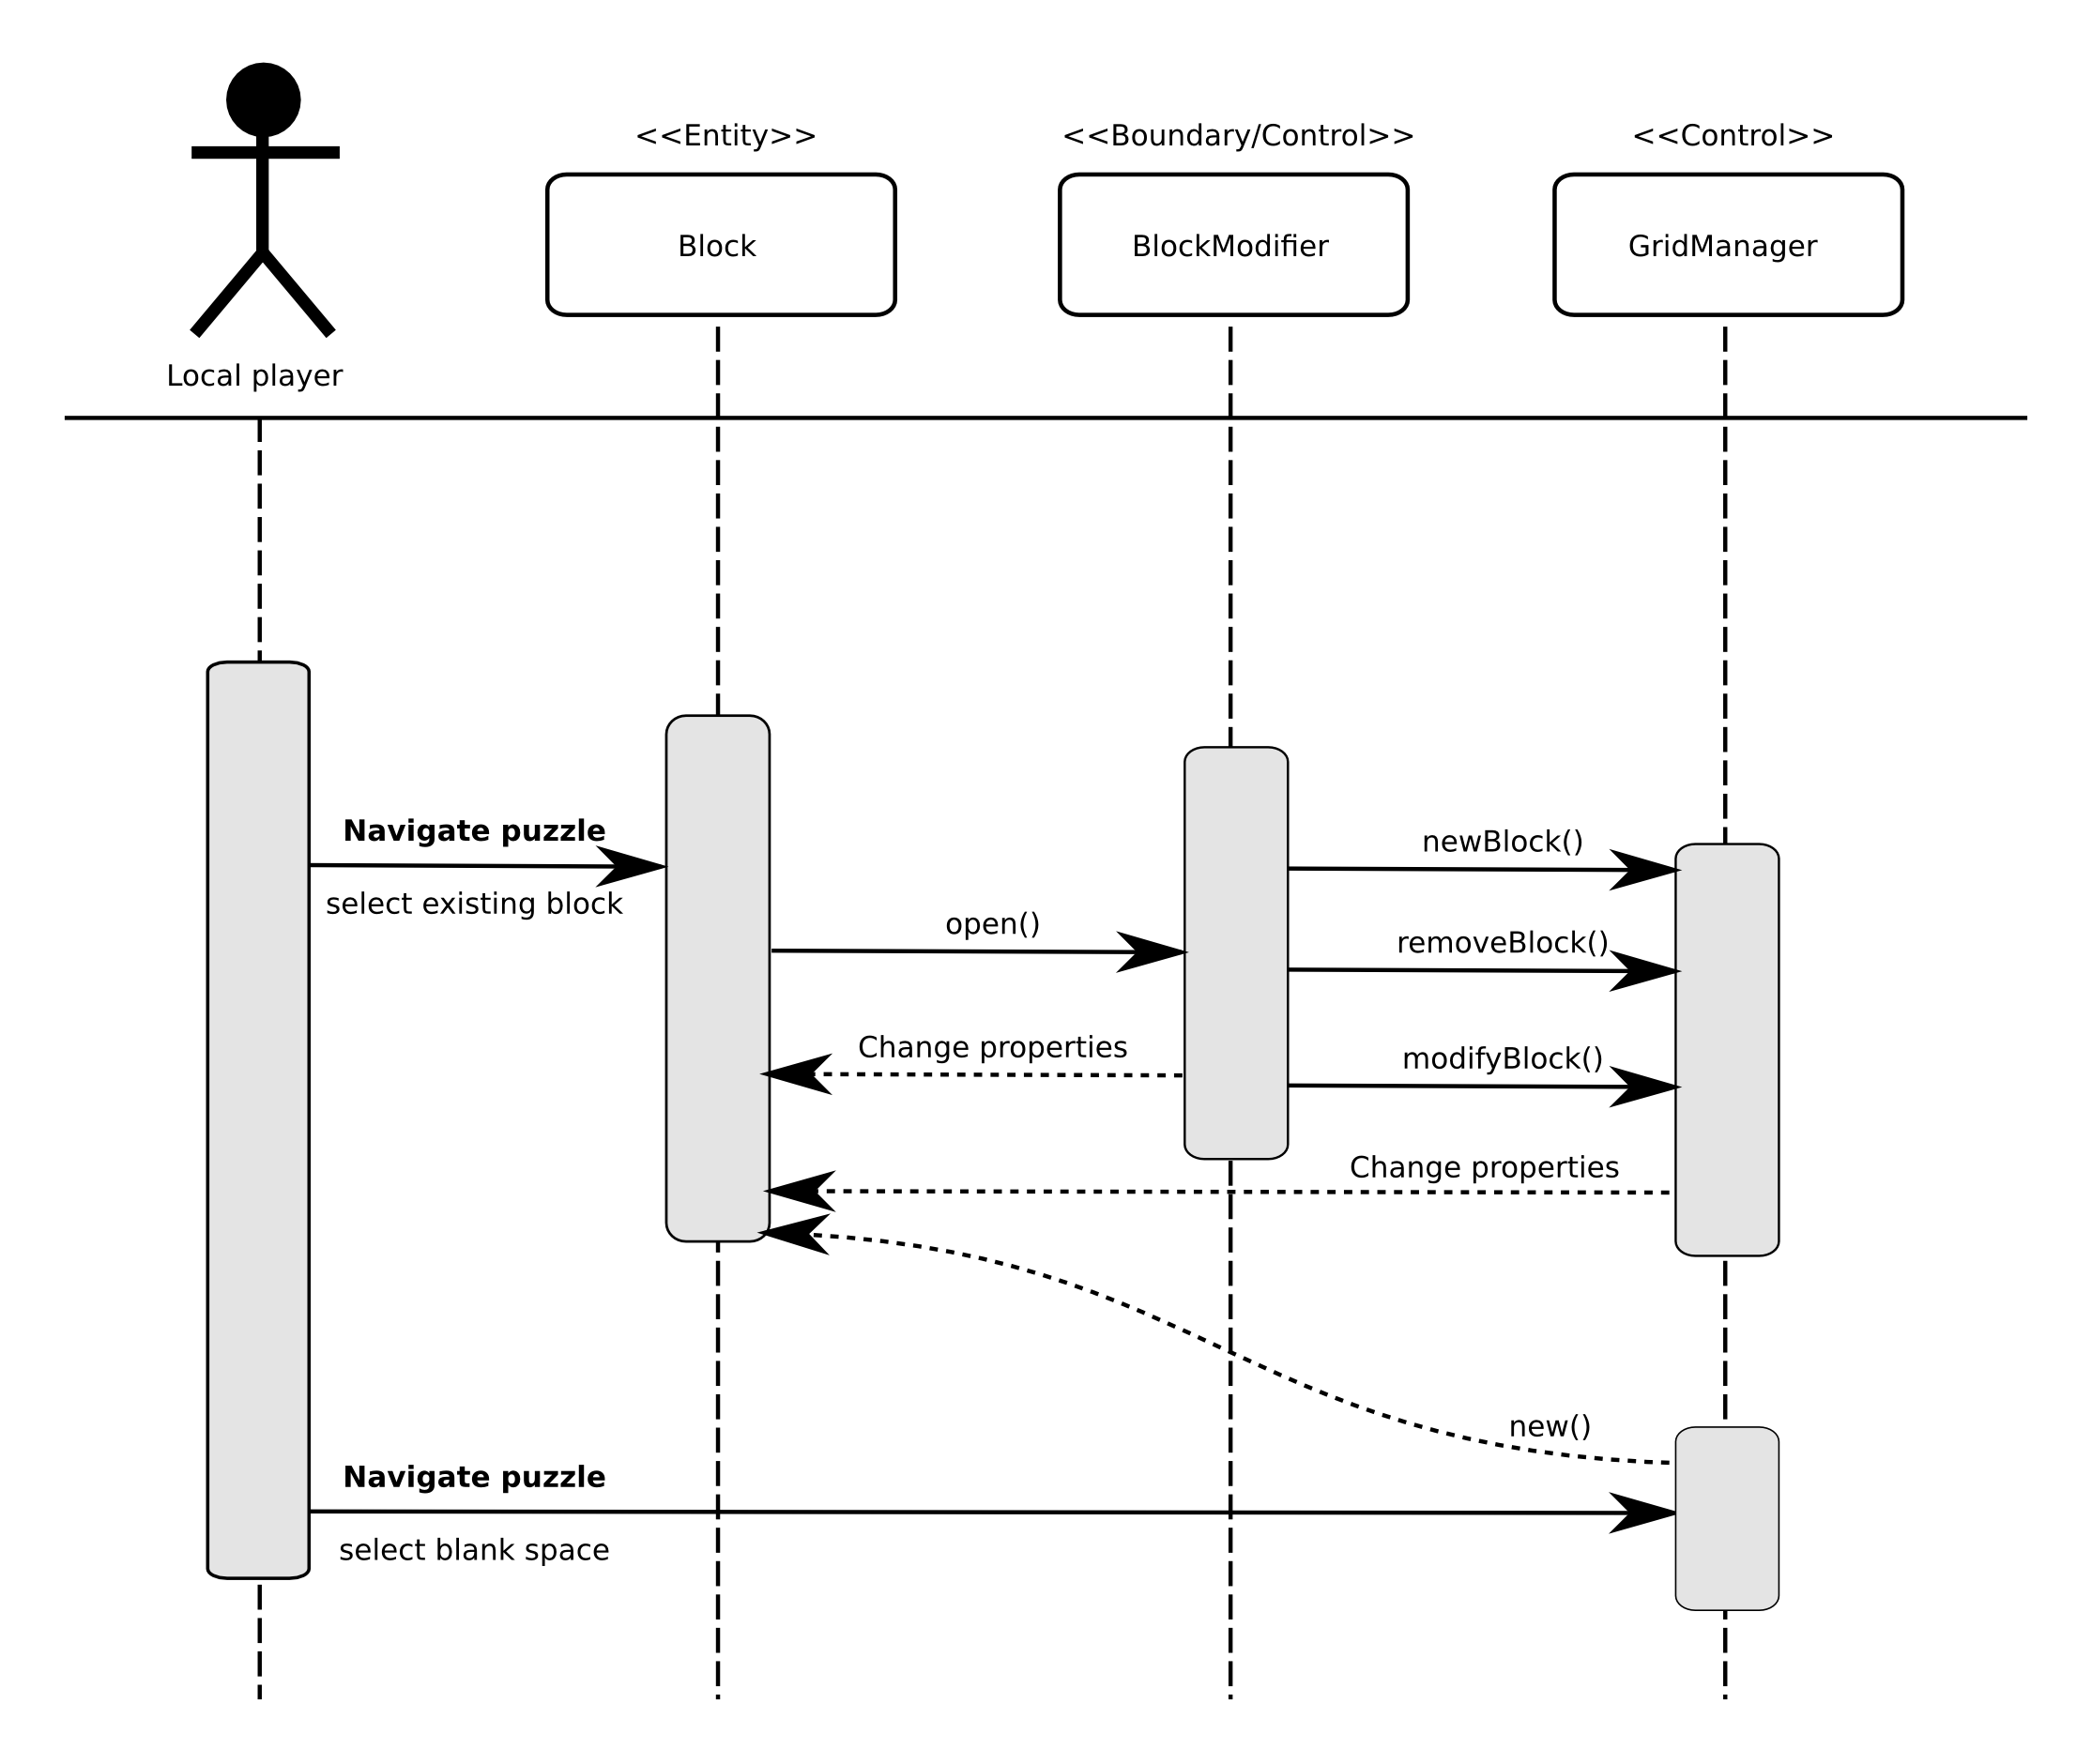
\includegraphics[width=6in]{sequence_edit.png}
        \caption{UML Sequence Diagram for editing or creating a puzzle}
    \end{figure}


    \begin{figure}[H]
        \centering
        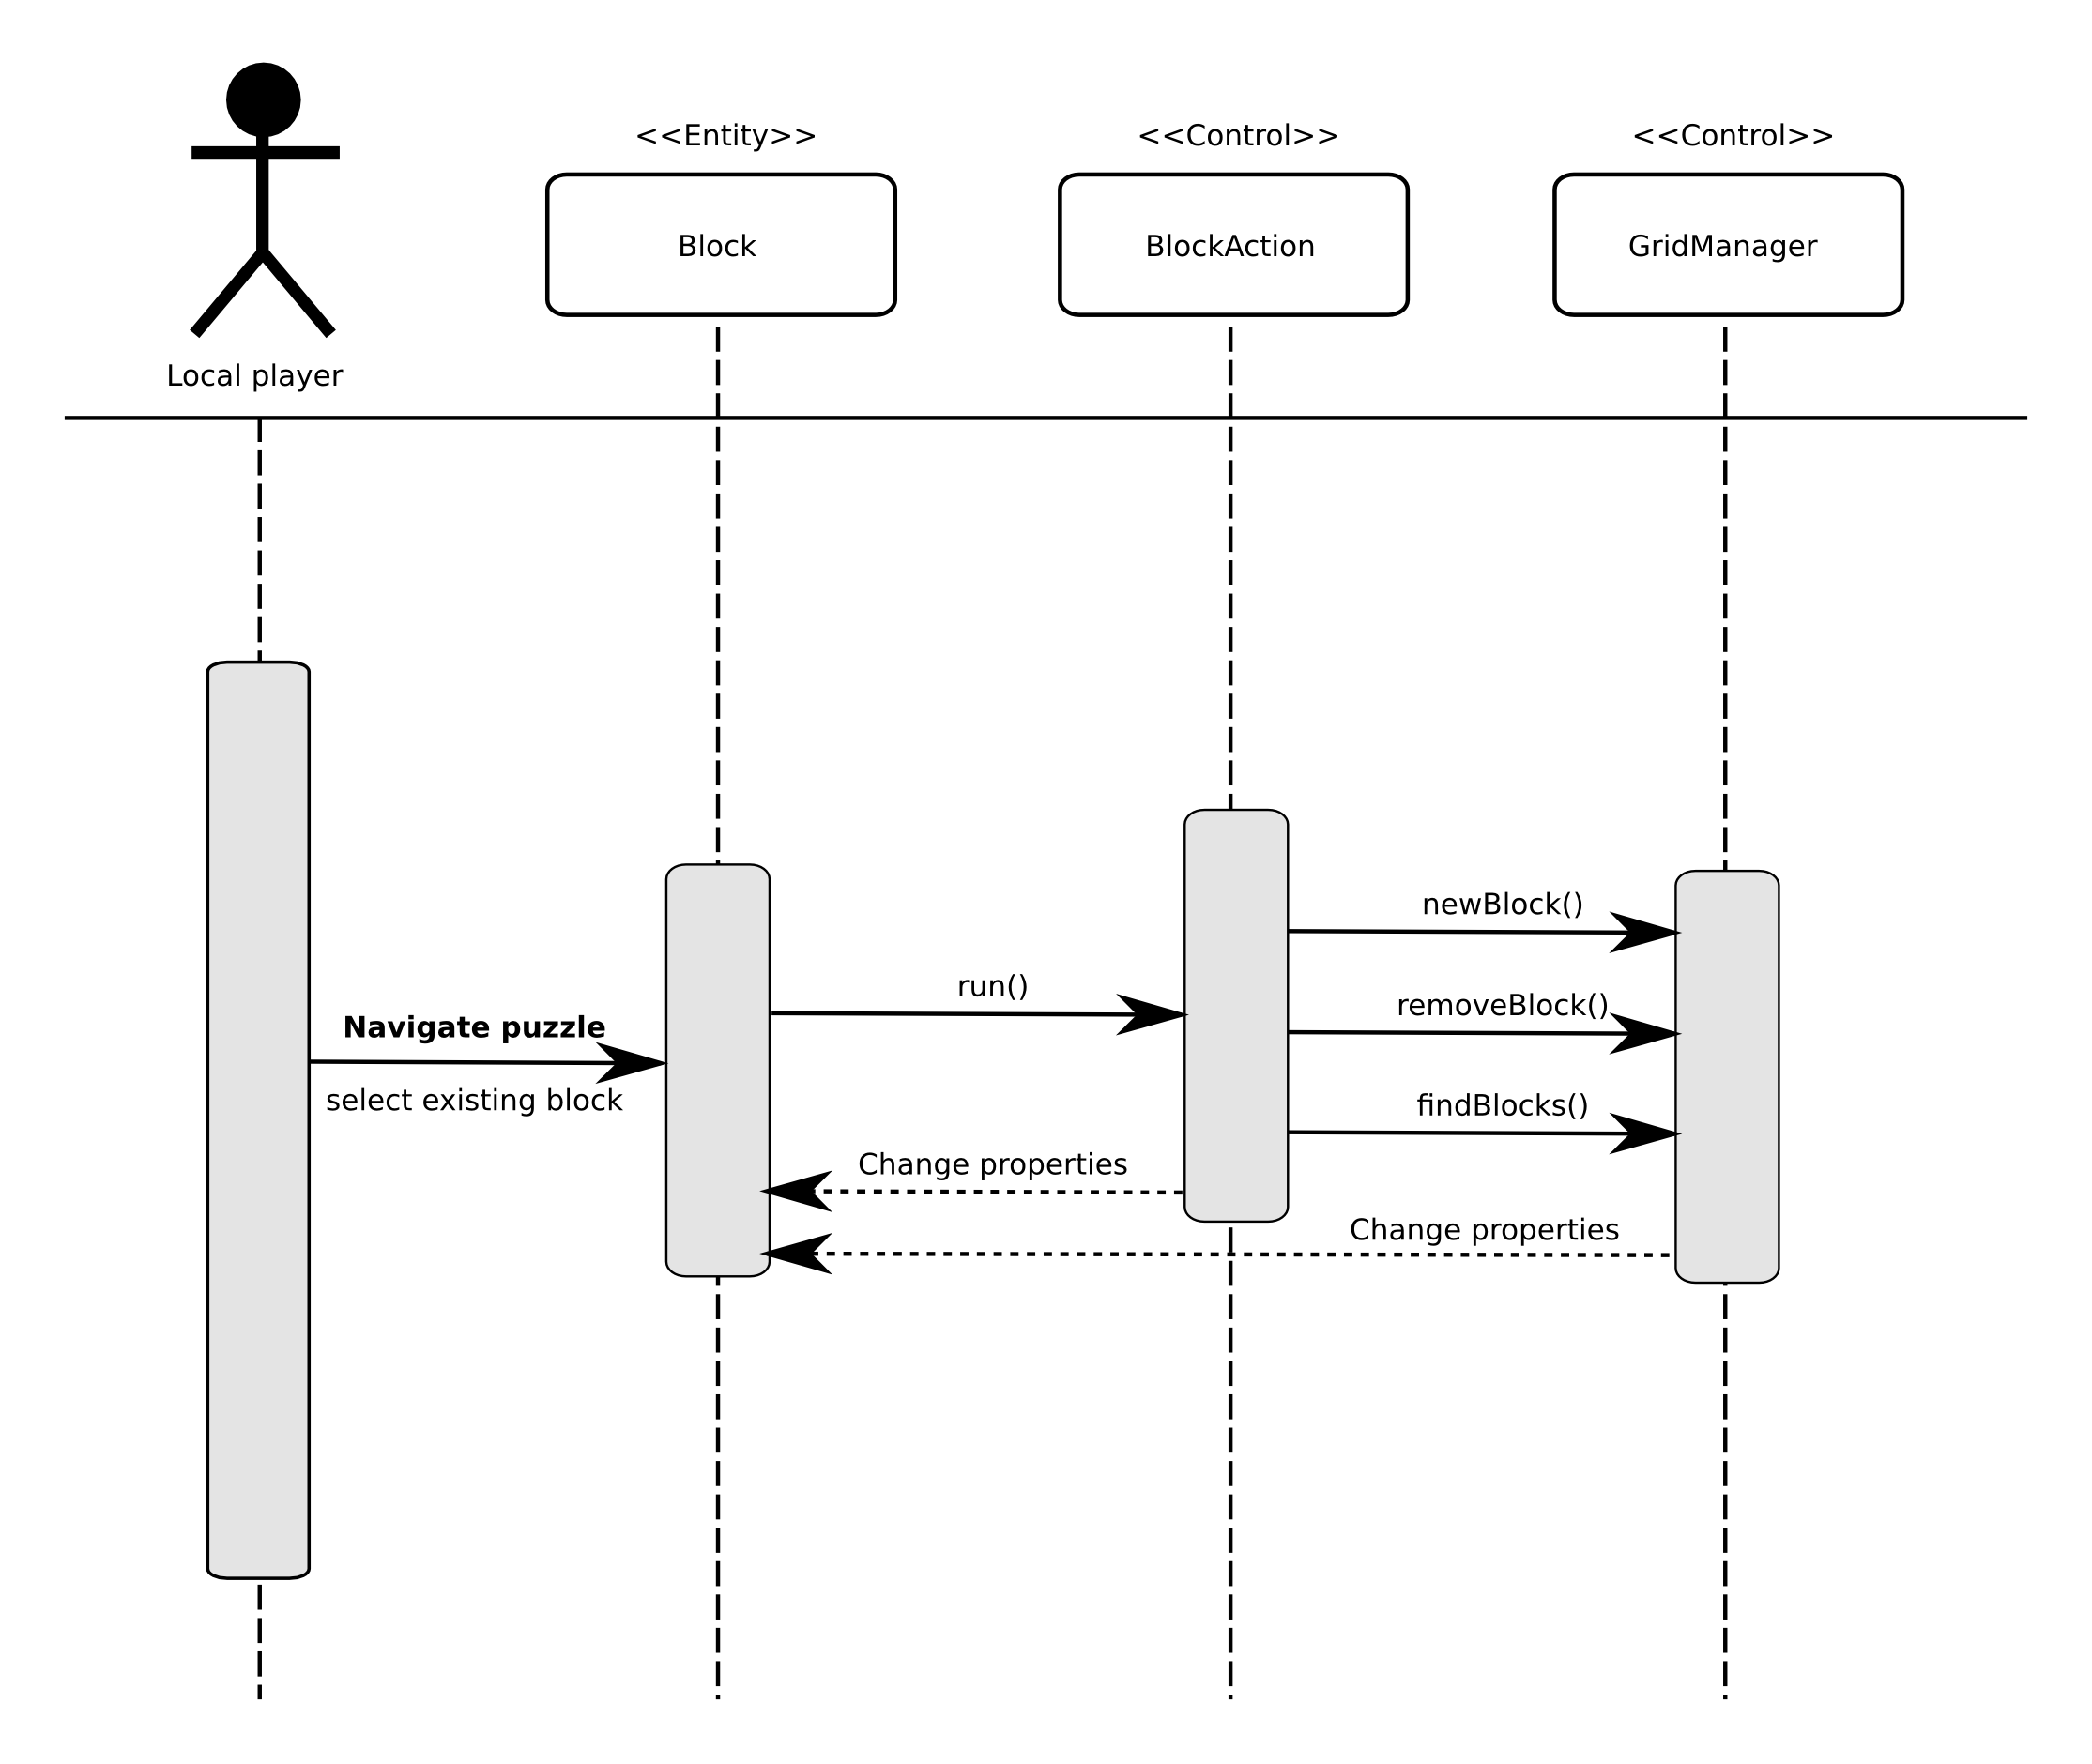
\includegraphics[width=6in]{sequence_solve.png}
        \caption{UML Sequence Diagram for the puzzle solving process}
    \end{figure}


    \begin{figure}[H]
        \centering
        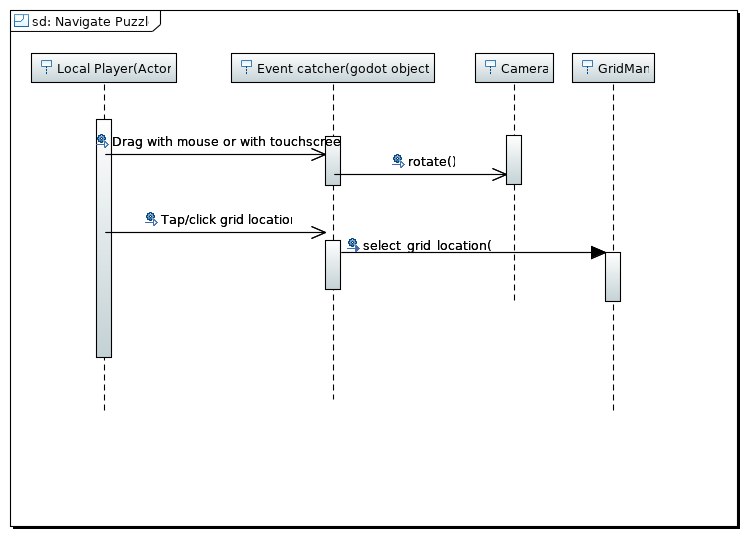
\includegraphics[width=6in]{sequence_navigate_puzzle.png}
        \caption{UML Sequence Diagram for navigating a puzzle in either edit or
        solve mode}
    \end{figure}


    \begin{figure}[H]
        \centering
        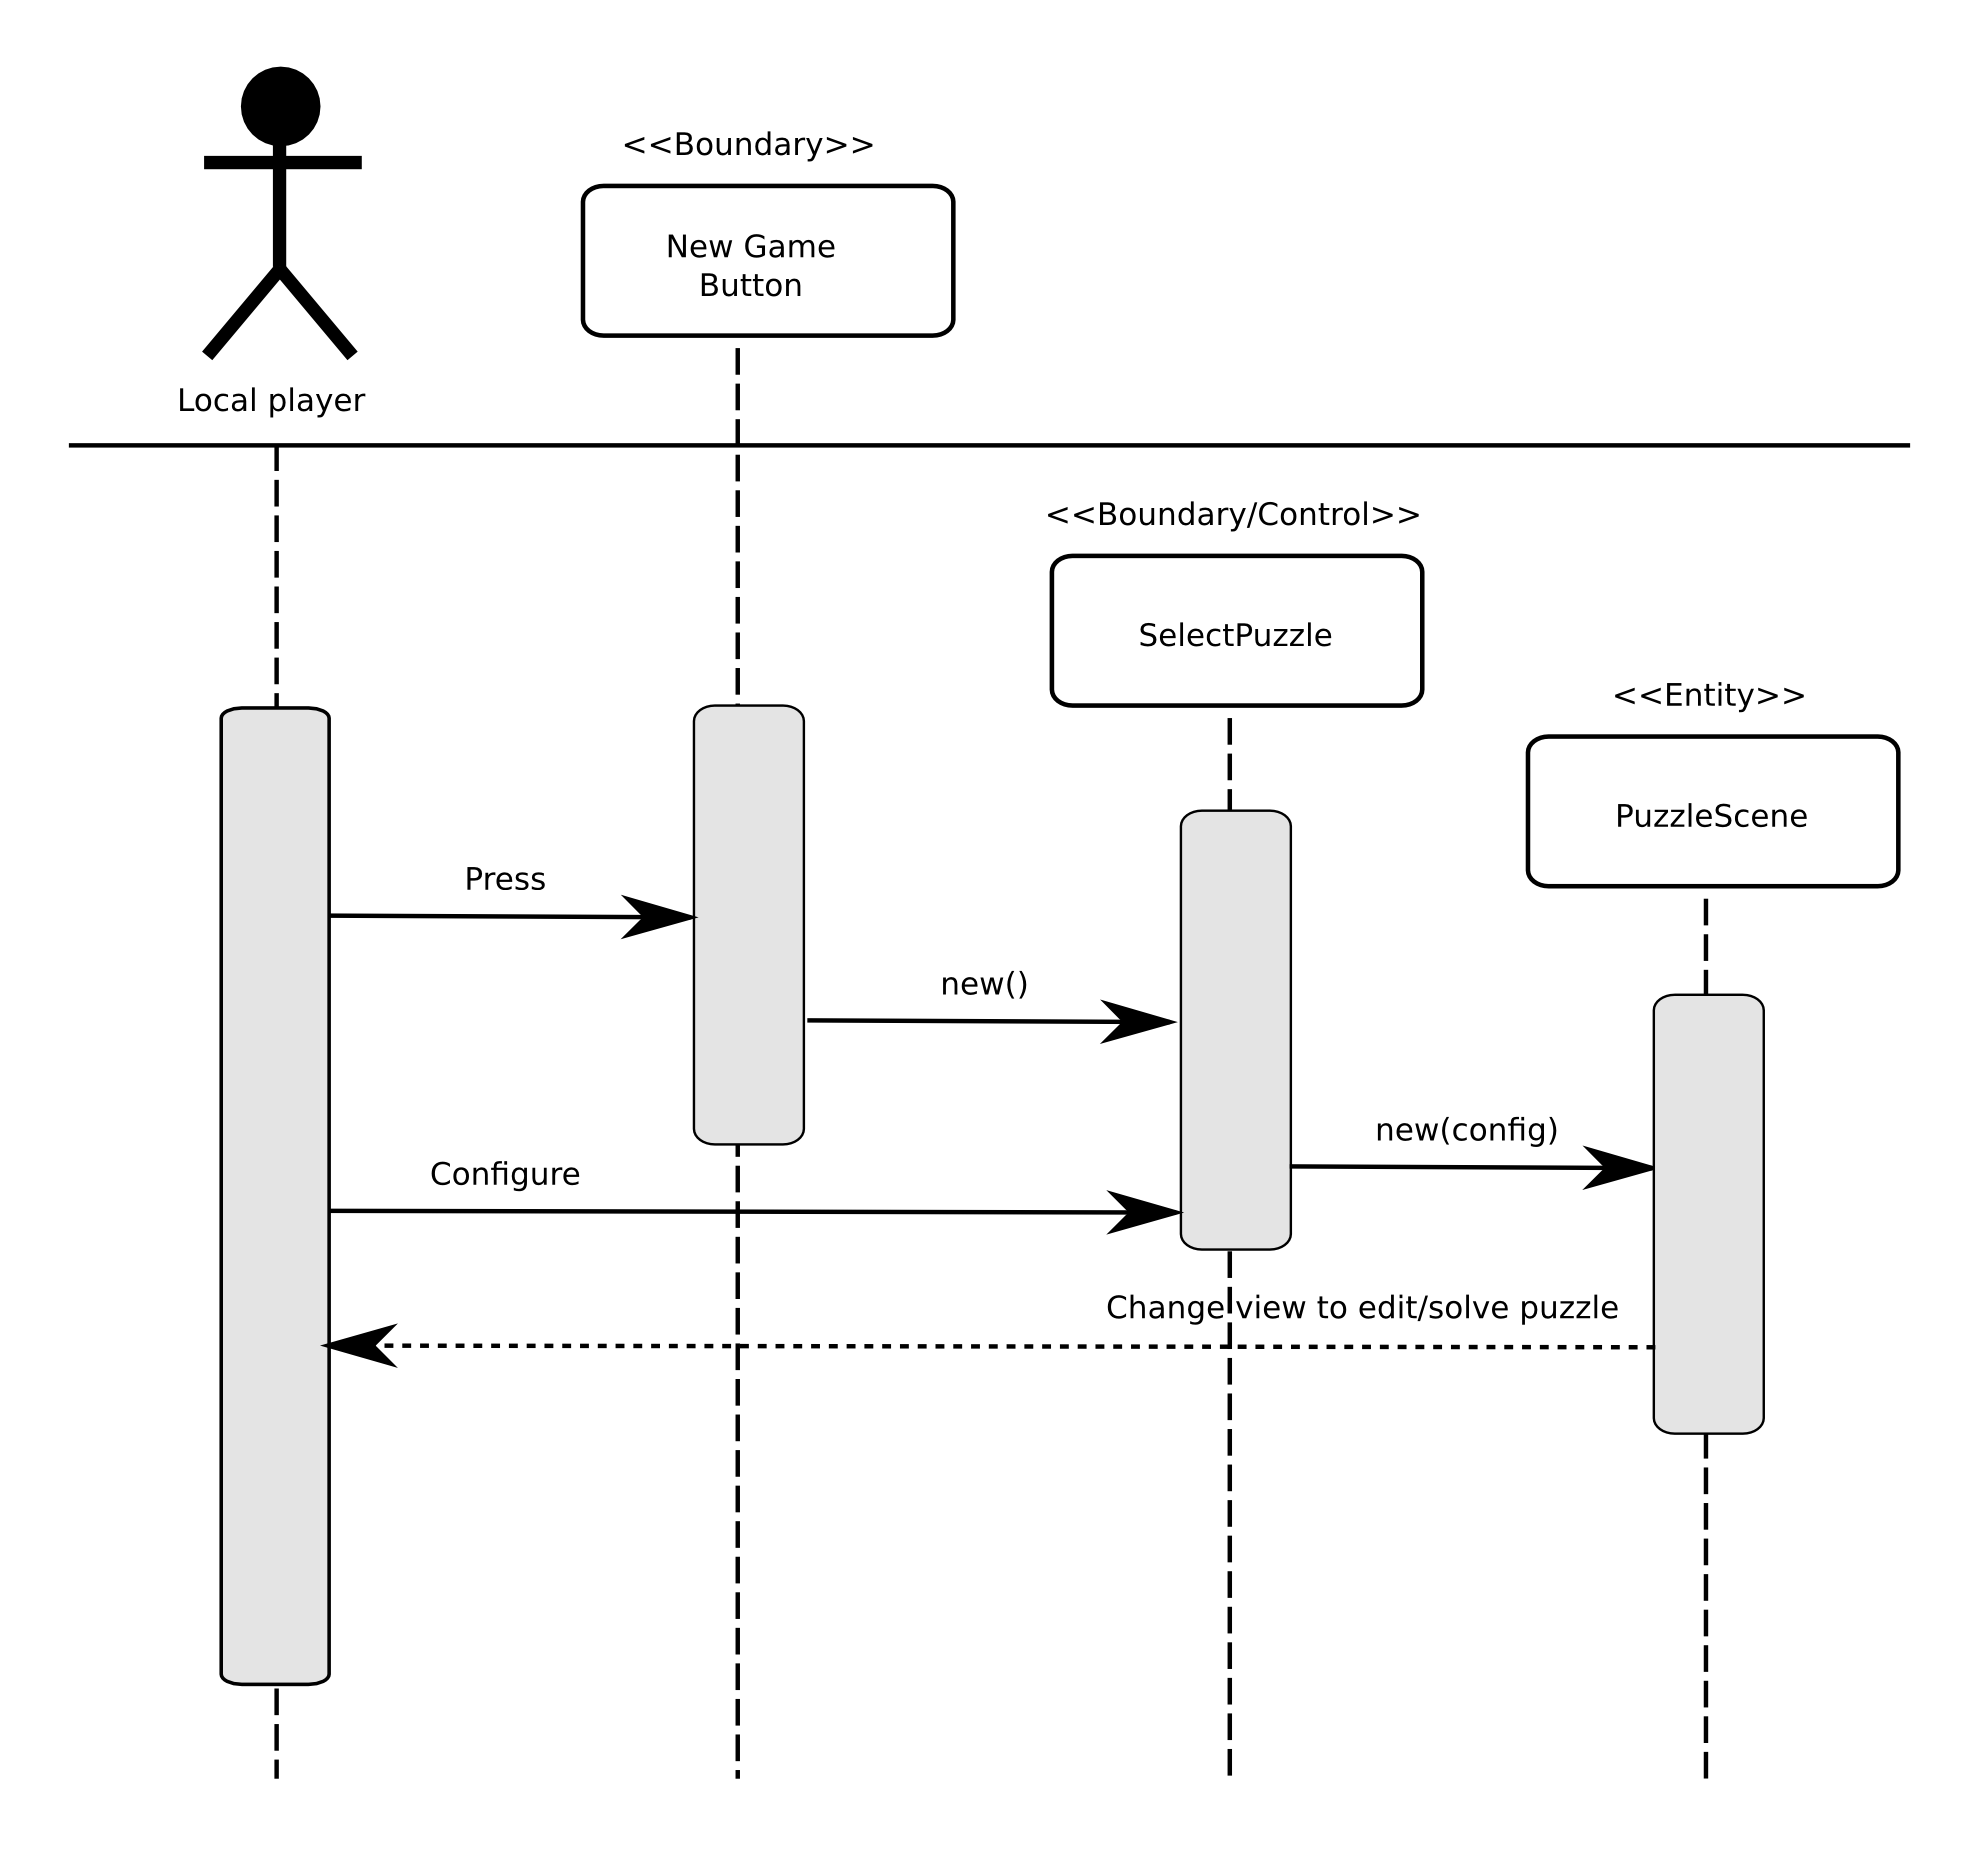
\includegraphics[width=6in]{sequence_offline_play.png}
        \caption{UML Sequence Diagram for an offline game}
    \end{figure}


    \begin{figure}[H]
        \centering
        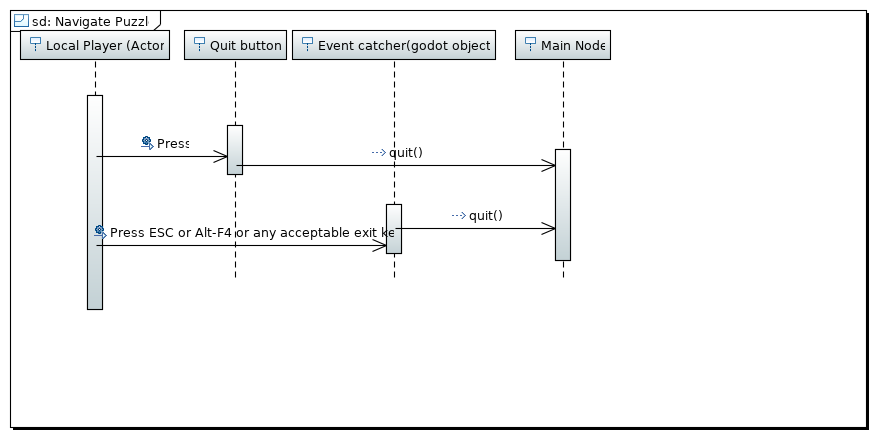
\includegraphics[width=6in]{sequence_quit.png}
        \caption{UML Sequence Diagram demonstrating game-shutdown}
    \end{figure}




\subsection{User Interface Analysis}\label{UI-analysis-CA}
The user interface in Anttris will follow the design of most simple game interfaces. It will include a main menu, configuration menu, play menu, editor interface and game interface. All of these will be connected to each other through the use of buttons on the screen that can be pressed with a mouse, a finger on a touch device and perhaps, with enough time, a game controller. Included below are flow diagrams for the user interface as well as initial design ideas for each individual interface.\\
\\
    \begin{figure}[H]
        \centering
        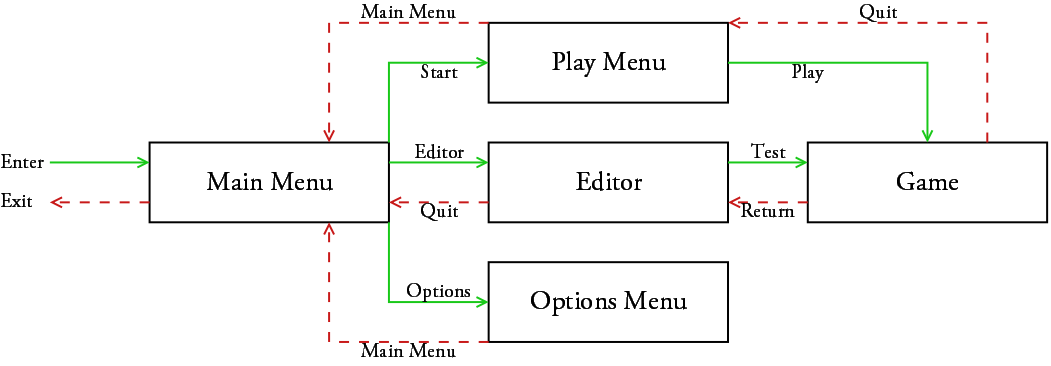
\includegraphics[width=6in]{UIFlow.png}
        \caption{Flow Diagram for UI}
    \end{figure}

% validation and criteria
\section{Validation and Criteria}\label{validation-BC}

% appendices
\section{Appendices}

\subsection{Project Status}\label{status-ST}

Much progress has been made. We have a working Javascript prototype, a
workable timeline for Scrum, and we have begun our first sprint. The
primary objective of this first sprint is to convert the prototype
into project for the Godot game engine \cite{godot:gameengine}.

Currently, we plan to have four sprints of two weeks duration each,
with weekends acting as slack days. Due to scheduling, the first
sprint is slightly longer than two weeks, so we plan to do more to
offset the projected downtime during spring break. Sean has taken on the job of coordinating the team as Scrum Master.

Our team also has solid organization and collaboration thanks to various tools, including Github for our git repositories \cite{github:site}, Zenhub for integrated Agile project management in Github \cite{zenhub:site}, Slack for team collaboration \cite{slack:site}, and Travis CI for continuous integration \cite{travis:site}.


\begin{table}[H]
\centering
\begin{tabular}{|l|l|l|l|l|}
\hline
& Sprint \#1 & Sprint \#2 & Sprint \#3 & Sprint \#4 \\ \hline
Date & 2/18 - 3/6 & 3/9 - 3/27 & 3/30 - 4/10 & 4/13 - end \\ \hline
Goals & Prototype & Get basic game working & Advanced features & Finish \\ \hline
Issues & none so far & Spring Break!?! & may not have time & hopefully none \\ \hline
&  &  &  &  \\ \hline
\end{tabular}
\caption{Scrum Timeline}
\label{timeline}
\end{table}


\bibliographystyle{abbrv}
\bibliography{team5-requirements-spec}
\end{document}







